\documentclass[11pt]{article}
\usepackage{cornell-notes}
\usepackage{mathtools}
\usepackage{needspace}
\usepackage{ragged2e}
\usepackage{adjustbox}
\usepackage{tikz}
\usetikzlibrary{arrows.meta,positioning}
\tcbuselibrary{most}
\geometry{letterpaper,margin=0.72in,headheight=15pt}
\setCornellCollection{Calculus Cornell Notes}
\setCornellUnitType{Chapter}
\setCornellUnitNumber{9}
\setCornellUnitTitle{Infinite Series}

\definecolor{Ink}{HTML}{17324D}
\definecolor{Teal}{HTML}{147D78}
\definecolor{Sky}{HTML}{DDEEF1}
\definecolor{Cue}{HTML}{EEF2F5}
\definecolor{Warm}{HTML}{FFF3D6}
\definecolor{Alert}{HTML}{9D3C32}
\definecolor{Green}{HTML}{276749}
\definecolor{Rule}{HTML}{AAB8C2}
\hypersetup{colorlinks=true,linkcolor=Ink,urlcolor=Teal,pdfborder={0 0 0}}
\setlength{\parindent}{0pt}
\setlength{\parskip}{4pt}
\setlist{nosep,leftmargin=*}
\titleformat{\section}{\Large\bfseries\color{Ink}}{}{0pt}{}[\color{Teal}\titlerule]
\titleformat{\subsection}{\large\bfseries\color{Teal}}{}{0pt}{}
\pagestyle{fancy}
\fancyhf{}
\fancyhead[L]{\small\color{Ink}\textsc{Cornell Notes}}
\fancyhead[R]{\small\color{Teal}\nouppercase{\leftmark}}
\fancyfoot[L]{\footnotesize\color{Ink}Active recall $\bullet$ Worked reasoning $\bullet$ Verification}
\fancyfoot[R]{\footnotesize\color{Ink}\thepage\ of \pageref*{LastPage}}
\renewcommand{\headrulewidth}{0.5pt}
\renewcommand{\footrulewidth}{0.4pt}
\newcolumntype{Y}{>{\RaggedRight\arraybackslash}X}
\newtcolorbox{orientationbox}{enhanced,breakable,colback=Sky,colframe=Teal,boxrule=0.7pt,arc=2mm,title=Chapter orientation,fonttitle=\bfseries}
\newtcolorbox{sectionsummarybox}{enhanced,breakable,colback=white,colframe=Teal,boxrule=0.6pt,arc=1.5mm,left=2mm,right=2mm,top=1mm,bottom=1mm,title=Section synthesis,fonttitle=\bfseries\color{Teal}}
\newtcolorbox{warningbox}{enhanced,breakable,colback=Warm,colframe=Alert,boxrule=0.7pt,arc=1.5mm,title=Common error audit,fonttitle=\bfseries}
\newtcolorbox{checkbox}{enhanced,breakable,colback=white,colframe=Green,boxrule=0.7pt,arc=1.5mm,title=Verification habit,fonttitle=\bfseries}
\newcommand{\cornellcuehead}{\rowcolor{Ink}\color{white}\bfseries Cue / recall prompt & \color{white}\bfseries Notes / reasoning \\\endhead}
\newcommand{\cornellcuerow}[2]{\rowcolor{Cue}#1 & #2 \\\addlinespace[3pt]}
\newcommand{\formula}[1]{\begin{tcolorbox}[colback=Sky,colframe=Teal,boxrule=0.5pt,arc=1mm,left=2mm,right=2mm,top=1mm,bottom=1mm]\centering\adjustbox{max width=0.97\linewidth}{$\displaystyle #1$}\end{tcolorbox}}

\title{Chapter 9: Infinite Series\\[2mm]\large Cornell Notes}
\author{}
\date{}
\hypersetup{pdftitle={Chapter 9: Infinite Series - Cornell Notes},pdfauthor={},pdfsubject={Calculus study notes},pdfkeywords={calculus, Cornell notes, active recall}}
\begin{document}
\maketitle
\thispagestyle{fancy}
\begin{orientationbox}
Analyze sequences and series, choose convergence tests, control approximation error, and represent functions by power and Taylor series. These notes follow the complete local section sequence (587--684) and emphasize definitions, governing results, strategy selection, and verifiable reasoning.
\end{orientationbox}

\section{Prerequisite map}
\begin{minipage}[t]{0.42\textwidth}
\textbf{Bring forward}
\begin{itemize}
\item Limits
\item Improper integrals
\item Derivative formulas
\item Algebra of polynomials
\end{itemize}
\end{minipage}\hfill
\begin{minipage}[t]{0.54\textwidth}
\textbf{Chapter flow}
\begin{center}
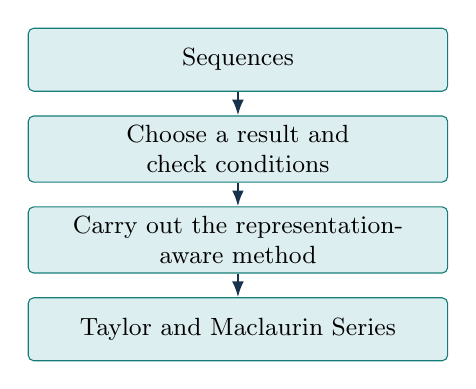
\begin{tikzpicture}[node distance=3mm, every node/.style={font=\small,align=center}, box/.style={draw=Teal,rounded corners=2pt,fill=Sky,minimum height=8mm,text width=0.42\textwidth}, arr/.style={-{Latex[length=2mm]},thick,draw=Ink}]
\node[box] (a) {Sequences};
\node[box,below=of a] (b) {Choose a result and check conditions};
\node[box,below=of b] (c) {Carry out the representation-aware method};
\node[box,below=of c] (d) {Taylor and Maclaurin Series};
\draw[arr] (a)--(b); \draw[arr] (b)--(c); \draw[arr] (c)--(d);
\end{tikzpicture}
\end{center}
\end{minipage}

\section{Learning objectives}
\begin{enumerate}
\item Explain the central objects and hypotheses in 9.1 and 9.10.
\item Translate among algebraic, graphical, numerical, and verbal representations.
\item Select an appropriate formula or theorem before beginning symbolic work.
\item Carry out multi-step calculations while preserving domain, sign, orientation, and units.
\item Diagnose common errors by testing assumptions and checking the result independently.
\item Synthesize the chapter's methods into a reusable problem-solving workflow.
\end{enumerate}

\section{9.1 Sequences}
\begin{longtable}{C N}\cornellcuehead
\cornellcuerow{What is the governing idea in 9.1?}{A sequence converges when its terms approach one finite value; monotone bounded sequences provide an important convergence mechanism.}
\cornellcuerow{Which result should be recalled?}{\formula{\lim_{n\to\infty}a_n=L}}
\cornellcuerow{How should a problem be organized?}{Simplify dominant terms, use limit laws or monotone-bounded reasoning, and distinguish the sequence from the set of its values.}
\cornellcuerow{What should be checked before accepting an answer?}{Confirm the hypotheses and domain, preserve units and orientation when relevant, and substitute or differentiate back into the defining relation.}
\end{longtable}
\begin{warningbox}A bounded sequence need not converge; oscillation can prevent a limit.\end{warningbox}
\begin{sectionsummarybox}A sequence converges when its terms approach one finite value; monotone bounded sequences provide an important convergence mechanism. The operational habit is to simplify dominant terms, use limit laws or monotone-bounded reasoning, and distinguish the sequence from the set of its values.\end{sectionsummarybox}
\section{9.2 Series and Convergence}
\begin{longtable}{C N}\cornellcuehead
\cornellcuerow{What is the governing idea in 9.2?}{A series converges when its sequence of partial sums converges; geometric and telescoping structures give exact benchmarks.}
\cornellcuerow{Which result should be recalled?}{\formula{\sum_{n=0}^{\infty}ar^n=\frac{a}{1-r}\quad(|r|<1)}}
\cornellcuerow{How should a problem be organized?}{Inspect $a_n	o0$, identify geometric or telescoping form, compute partial sums when possible, and state the starting index.}
\cornellcuerow{What should be checked before accepting an answer?}{Confirm the hypotheses and domain, preserve units and orientation when relevant, and substitute or differentiate back into the defining relation.}
\end{longtable}
\begin{warningbox}$a_n	o0$ is necessary but not sufficient for series convergence.\end{warningbox}
\begin{sectionsummarybox}A series converges when its sequence of partial sums converges; geometric and telescoping structures give exact benchmarks. The operational habit is to inspect $a_n	o0$, identify geometric or telescoping form, compute partial sums when possible, and state the starting index.\end{sectionsummarybox}
\section{9.3 The Integral Test and p-Series}
\begin{longtable}{C N}\cornellcuehead
\cornellcuerow{What is the governing idea in 9.3?}{Positive decreasing terms can be compared with an improper integral; $p$-series establish a threshold at $p=1$.}
\cornellcuerow{Which result should be recalled?}{\formula{\sum\frac1{n^p}\text{ converges iff }p>1}}
\cornellcuerow{How should a problem be organized?}{Verify positivity, continuity, and decrease for the associated function, then apply the integral test or recognize a $p$-series.}
\cornellcuerow{What should be checked before accepting an answer?}{Confirm the hypotheses and domain, preserve units and orientation when relevant, and substitute or differentiate back into the defining relation.}
\end{longtable}
\begin{warningbox}Using the integral test without eventual decrease or reversing the $p$ threshold invalidates the conclusion.\end{warningbox}
\begin{sectionsummarybox}Positive decreasing terms can be compared with an improper integral; $p$-series establish a threshold at $p=1$. The operational habit is to verify positivity, continuity, and decrease for the associated function, then apply the integral test or recognize a $p$-series.\end{sectionsummarybox}
\section{9.4 Comparisons of Series}
\begin{longtable}{C N}\cornellcuehead
\cornellcuerow{What is the governing idea in 9.4?}{Direct and limit comparison transfer convergence behavior between positive-term series of comparable size.}
\cornellcuerow{Which result should be recalled?}{\formula{\lim_{n\to\infty}\frac{a_n}{b_n}=c,\quad 0<c<\infty}}
\cornellcuerow{How should a problem be organized?}{Choose a benchmark from dominant terms, decide which inequality direction would prove the desired result, and verify positivity eventually.}
\cornellcuerow{What should be checked before accepting an answer?}{Confirm the hypotheses and domain, preserve units and orientation when relevant, and substitute or differentiate back into the defining relation.}
\end{longtable}
\begin{warningbox}Comparing in the wrong direction cannot prove convergence or divergence even if the inequality is true.\end{warningbox}
\begin{sectionsummarybox}Direct and limit comparison transfer convergence behavior between positive-term series of comparable size. The operational habit is to choose a benchmark from dominant terms, decide which inequality direction would prove the desired result, and verify positivity eventually.\end{sectionsummarybox}
\section{9.5 Alternating Series}
\begin{longtable}{C N}\cornellcuehead
\cornellcuerow{What is the governing idea in 9.5?}{Alternating series converge when magnitudes decrease to zero, with truncation error bounded by the first omitted term.}
\cornellcuerow{Which result should be recalled?}{\formula{|R_N|\le b_{N+1}\quad\text{for }\sum(-1)^n b_n}}
\cornellcuerow{How should a problem be organized?}{Check eventual decrease and zero limit, distinguish conditional from absolute convergence, and solve the error bound for $N$.}
\cornellcuerow{What should be checked before accepting an answer?}{Confirm the hypotheses and domain, preserve units and orientation when relevant, and substitute or differentiate back into the defining relation.}
\end{longtable}
\begin{warningbox}Alternation alone is insufficient, and the next-term bound does not apply to arbitrary signed series.\end{warningbox}
\begin{sectionsummarybox}Alternating series converge when magnitudes decrease to zero, with truncation error bounded by the first omitted term. The operational habit is to check eventual decrease and zero limit, distinguish conditional from absolute convergence, and solve the error bound for $N$.\end{sectionsummarybox}
\section{9.6 The Ratio and Root Tests}
\begin{longtable}{C N}\cornellcuehead
\cornellcuerow{What is the governing idea in 9.6?}{Ratio and root tests detect exponential-scale behavior and are especially effective with factorials or powers.}
\cornellcuerow{Which result should be recalled?}{\formula{L=\lim\left|\frac{a_{n+1}}{a_n}\right|:\ L<1\Rightarrow\text{absolute convergence}}}
\cornellcuerow{How should a problem be organized?}{Simplify the ratio or $n$th root, evaluate the limit, and choose another test when $L=1$.}
\cornellcuerow{What should be checked before accepting an answer?}{Confirm the hypotheses and domain, preserve units and orientation when relevant, and substitute or differentiate back into the defining relation.}
\end{longtable}
\begin{warningbox}The tests are inconclusive at $L=1$; they do not prove divergence there.\end{warningbox}
\begin{sectionsummarybox}Ratio and root tests detect exponential-scale behavior and are especially effective with factorials or powers. The operational habit is to simplify the ratio or $n$th root, evaluate the limit, and choose another test when $L=1$.\end{sectionsummarybox}
\section{9.7 Taylor Polynomials and Approximations}
\begin{longtable}{C N}\cornellcuehead
\cornellcuerow{What is the governing idea in 9.7?}{A Taylor polynomial matches derivatives of a function at a center and gives a local approximation with controllable remainder.}
\cornellcuerow{Which result should be recalled?}{\formula{P_n(x)=\sum_{k=0}^{n}\frac{f^{(k)}(c)}{k!}(x-c)^k}}
\cornellcuerow{How should a problem be organized?}{Choose center and degree, compute derivatives systematically, and estimate the remainder on an interval containing $c$ and $x$.}
\cornellcuerow{What should be checked before accepting an answer?}{Confirm the hypotheses and domain, preserve units and orientation when relevant, and substitute or differentiate back into the defining relation.}
\end{longtable}
\begin{warningbox}Small polynomial degree is not automatically accurate far from the center.\end{warningbox}
\begin{sectionsummarybox}A Taylor polynomial matches derivatives of a function at a center and gives a local approximation with controllable remainder. The operational habit is to choose center and degree, compute derivatives systematically, and estimate the remainder on an interval containing $c$ and $x$.\end{sectionsummarybox}
\section{9.8 Power Series}
\begin{longtable}{C N}\cornellcuehead
\cornellcuerow{What is the governing idea in 9.8?}{A power series converges inside a radius around its center, diverges outside, and requires separate endpoint tests.}
\cornellcuerow{Which result should be recalled?}{\formula{\sum_{n=0}^{\infty}a_n(x-c)^n,\qquad |x-c|<R}}
\cornellcuerow{How should a problem be organized?}{Use ratio or root test for $R$, solve the resulting inequality, and test each endpoint with an ordinary series test.}
\cornellcuerow{What should be checked before accepting an answer?}{Confirm the hypotheses and domain, preserve units and orientation when relevant, and substitute or differentiate back into the defining relation.}
\end{longtable}
\begin{warningbox}Including endpoints automatically is the classic interval-of-convergence error.\end{warningbox}
\begin{sectionsummarybox}A power series converges inside a radius around its center, diverges outside, and requires separate endpoint tests. The operational habit is to use ratio or root test for $R$, solve the resulting inequality, and test each endpoint with an ordinary series test.\end{sectionsummarybox}
\section{9.9 Representation of Functions by Power Series}
\begin{longtable}{C N}\cornellcuehead
\cornellcuerow{What is the governing idea in 9.9?}{Known series can be differentiated, integrated, substituted, or combined within their intervals of convergence.}
\cornellcuerow{Which result should be recalled?}{\formula{\frac1{1-x}=\sum_{n=0}^{\infty}x^n\quad(|x|<1)}}
\cornellcuerow{How should a problem be organized?}{Start from a trusted base series, transform coefficients and powers carefully, and update the interval and endpoint analysis.}
\cornellcuerow{What should be checked before accepting an answer?}{Confirm the hypotheses and domain, preserve units and orientation when relevant, and substitute or differentiate back into the defining relation.}
\end{longtable}
\begin{warningbox}Algebraic transformations may change endpoint behavior even when the radius remains easy to track.\end{warningbox}
\begin{sectionsummarybox}Known series can be differentiated, integrated, substituted, or combined within their intervals of convergence. The operational habit is to start from a trusted base series, transform coefficients and powers carefully, and update the interval and endpoint analysis.\end{sectionsummarybox}
\section{9.10 Taylor and Maclaurin Series}
\begin{longtable}{C N}\cornellcuehead
\cornellcuerow{What is the governing idea in 9.10?}{The infinite Taylor series represents a function where its remainder tends to zero, not merely because all derivatives exist.}
\cornellcuerow{Which result should be recalled?}{\formula{f(x)=\sum_{n=0}^{\infty}\frac{f^{(n)}(c)}{n!}(x-c)^n}}
\cornellcuerow{How should a problem be organized?}{Find the derivative pattern, write a general coefficient, determine convergence, and justify equality using a remainder argument.}
\cornellcuerow{What should be checked before accepting an answer?}{Confirm the hypotheses and domain, preserve units and orientation when relevant, and substitute or differentiate back into the defining relation.}
\end{longtable}
\begin{warningbox}A Taylor series may converge without converging to the original function outside the justified region.\end{warningbox}
\begin{sectionsummarybox}The infinite Taylor series represents a function where its remainder tends to zero, not merely because all derivatives exist. The operational habit is to find the derivative pattern, write a general coefficient, determine convergence, and justify equality using a remainder argument.\end{sectionsummarybox}

\section{Definitions and theorem register}
\small
\begin{longtable}{@{}>{\RaggedRight\arraybackslash}p{0.24\textwidth}>{\RaggedRight\arraybackslash}p{0.40\textwidth}>{\RaggedRight\arraybackslash}p{0.29\textwidth}@{}}
\toprule
\textbf{Topic} & \textbf{Meaning and conditions} & \textbf{Canonical form}\\
\midrule\endhead
9.1 Sequences & A sequence converges when its terms approach one finite value; monotone bounded sequences provide an important convergence mechanism. & \adjustbox{max width=\linewidth}{\(\displaystyle \lim_{n\to\infty}a_n=L\)} \\\addlinespace[2pt]
9.2 Series and Convergence & A series converges when its sequence of partial sums converges; geometric and telescoping structures give exact benchmarks. & \adjustbox{max width=\linewidth}{\(\displaystyle \sum_{n=0}^{\infty}ar^n=\frac{a}{1-r}\quad(|r|<1)\)} \\\addlinespace[2pt]
9.3 The Integral Test and p-Series & Positive decreasing terms can be compared with an improper integral; $p$-series establish a threshold at $p=1$. & \adjustbox{max width=\linewidth}{\(\displaystyle \sum\frac1{n^p}\text{ converges iff }p>1\)} \\\addlinespace[2pt]
9.4 Comparisons of Series & Direct and limit comparison transfer convergence behavior between positive-term series of comparable size. & \adjustbox{max width=\linewidth}{\(\displaystyle \lim_{n\to\infty}\frac{a_n}{b_n}=c,\quad 0<c<\infty\)} \\\addlinespace[2pt]
9.5 Alternating Series & Alternating series converge when magnitudes decrease to zero, with truncation error bounded by the first omitted term. & \adjustbox{max width=\linewidth}{\(\displaystyle |R_N|\le b_{N+1}\quad\text{for }\sum(-1)^n b_n\)} \\\addlinespace[2pt]
9.6 The Ratio and Root Tests & Ratio and root tests detect exponential-scale behavior and are especially effective with factorials or powers. & \adjustbox{max width=\linewidth}{\(\displaystyle L=\lim\left|\frac{a_{n+1}}{a_n}\right|:\ L<1\Rightarrow\text{absolute convergence}\)} \\\addlinespace[2pt]
9.7 Taylor Polynomials and Approximations & A Taylor polynomial matches derivatives of a function at a center and gives a local approximation with controllable remainder. & \adjustbox{max width=\linewidth}{\(\displaystyle P_n(x)=\sum_{k=0}^{n}\frac{f^{(k)}(c)}{k!}(x-c)^k\)} \\\addlinespace[2pt]
9.8 Power Series & A power series converges inside a radius around its center, diverges outside, and requires separate endpoint tests. & \adjustbox{max width=\linewidth}{\(\displaystyle \sum_{n=0}^{\infty}a_n(x-c)^n,\qquad |x-c|<R\)} \\\addlinespace[2pt]
9.9 Representation of Functions by Power Series & Known series can be differentiated, integrated, substituted, or combined within their intervals of convergence. & \adjustbox{max width=\linewidth}{\(\displaystyle \frac1{1-x}=\sum_{n=0}^{\infty}x^n\quad(|x|<1)\)} \\\addlinespace[2pt]
9.10 Taylor and Maclaurin Series & The infinite Taylor series represents a function where its remainder tends to zero, not merely because all derivatives exist. & \adjustbox{max width=\linewidth}{\(\displaystyle f(x)=\sum_{n=0}^{\infty}\frac{f^{(n)}(c)}{n!}(x-c)^n\)} \\\addlinespace[2pt]
\bottomrule
\end{longtable}
\normalsize

\section{Formula and method sheet}
\small
\begin{longtable}{@{}>{\RaggedRight\arraybackslash}p{0.08\textwidth}>{\RaggedRight\arraybackslash}p{0.48\textwidth}>{\RaggedRight\arraybackslash}p{0.37\textwidth}@{}}
\toprule
\textbf{Sec.} & \textbf{Method sequence} & \textbf{Stop-and-check trigger}\\
\midrule\endhead
9.1 & Simplify dominant terms, use limit laws or monotone-bounded reasoning, and distinguish the sequence from the set of its values. & A bounded sequence need not converge; oscillation can prevent a limit. \\\addlinespace[2pt]
9.2 & Inspect $a_n o0$, identify geometric or telescoping form, compute partial sums when possible, and state the starting index. & $a_n o0$ is necessary but not sufficient for series convergence. \\\addlinespace[2pt]
9.3 & Verify positivity, continuity, and decrease for the associated function, then apply the integral test or recognize a $p$-series. & Using the integral test without eventual decrease or reversing the $p$ threshold invalidates the conclusion. \\\addlinespace[2pt]
9.4 & Choose a benchmark from dominant terms, decide which inequality direction would prove the desired result, and verify positivity eventually. & Comparing in the wrong direction cannot prove convergence or divergence even if the inequality is true. \\\addlinespace[2pt]
9.5 & Check eventual decrease and zero limit, distinguish conditional from absolute convergence, and solve the error bound for $N$. & Alternation alone is insufficient, and the next-term bound does not apply to arbitrary signed series. \\\addlinespace[2pt]
9.6 & Simplify the ratio or $n$th root, evaluate the limit, and choose another test when $L=1$. & The tests are inconclusive at $L=1$; they do not prove divergence there. \\\addlinespace[2pt]
9.7 & Choose center and degree, compute derivatives systematically, and estimate the remainder on an interval containing $c$ and $x$. & Small polynomial degree is not automatically accurate far from the center. \\\addlinespace[2pt]
9.8 & Use ratio or root test for $R$, solve the resulting inequality, and test each endpoint with an ordinary series test. & Including endpoints automatically is the classic interval-of-convergence error. \\\addlinespace[2pt]
9.9 & Start from a trusted base series, transform coefficients and powers carefully, and update the interval and endpoint analysis. & Algebraic transformations may change endpoint behavior even when the radius remains easy to track. \\\addlinespace[2pt]
9.10 & Find the derivative pattern, write a general coefficient, determine convergence, and justify equality using a remainder argument. & A Taylor series may converge without converging to the original function outside the justified region. \\\addlinespace[2pt]
\bottomrule
\end{longtable}
\normalsize

\section{Common errors and diagnostic checks}
\begin{warningbox}
\begin{itemize}
\item \textbf{9.1:} A bounded sequence need not converge; oscillation can prevent a limit.
\item \textbf{9.2:} $a_n	o0$ is necessary but not sufficient for series convergence.
\item \textbf{9.3:} Using the integral test without eventual decrease or reversing the $p$ threshold invalidates the conclusion.
\item \textbf{9.4:} Comparing in the wrong direction cannot prove convergence or divergence even if the inequality is true.
\item \textbf{9.5:} Alternation alone is insufficient, and the next-term bound does not apply to arbitrary signed series.
\item \textbf{9.6:} The tests are inconclusive at $L=1$; they do not prove divergence there.
\item \textbf{9.7:} Small polynomial degree is not automatically accurate far from the center.
\item \textbf{9.8:} Including endpoints automatically is the classic interval-of-convergence error.
\item \textbf{9.9:} Algebraic transformations may change endpoint behavior even when the radius remains easy to track.
\item \textbf{9.10:} A Taylor series may converge without converging to the original function outside the justified region.
\end{itemize}
\end{warningbox}
\begin{checkbox}
Before accepting any result: state the relevant domain; check theorem hypotheses; estimate sign and scale; preserve units and orientation; and verify by substitution, differentiation, a limiting case, or a second representation.
\end{checkbox}

\section{Chapter synthesis}
Analyze sequences and series, choose convergence tests, control approximation error, and represent functions by power and Taylor series. The chapter begins with \textbf{Sequences} and culminates in \textbf{Taylor and Maclaurin Series}. Across the sequence, the most reliable workflow is to identify the mathematical object, choose a representation, state the governing result with its hypotheses, compute without dropping restrictions, and audit the answer against the original definition. Series reasoning separates term limits, partial-sum convergence, test hypotheses, endpoint behavior, and approximation error; no single test replaces that decision tree.

\section{Self-test questions}
\begin{enumerate}
\item Explain the central distinction or object in 9.1, using both words and notation.
\item State the main formula or result from 9.2 and identify every hypothesis or restriction needed for its use.
\item Describe the problem-solving procedure for 9.3. What is the strongest independent check?
\item Compare the roles of Sequences and Taylor and Maclaurin Series within this chapter.
\item Reconstruct the governing formula for 9.4 from its geometric or analytic meaning.
\item Choose one method in the chapter and explain how its output should be interpreted, including units or orientation when applicable.
\item Scenario: A student working on 9.1 produces a polished calculation but makes this error: A bounded sequence need not converge; oscillation can prevent a limit. Diagnose the earliest invalid step and repair the workflow.
\item Scenario: A solution in 9.2 quotes the displayed formula without checking conditions. Which conditions must be checked, and what could fail if they are absent?
\item Construct a concept map linking a representation, a governing result, a computation, and a verification check from this chapter.
\item Design a two-part test for mastery: one conceptual prompt and one calculation. State what evidence would count as a complete answer.
\end{enumerate}

\Needspace{8\baselineskip}
\section{Answer key}
\small
\begin{enumerate}
\item A complete response identifies A sequence converges when its terms approach one finite value; monotone bounded sequences provide an important convergence mechanism. It should connect that meaning to \(\lim_{n\to\infty}a_n=L\) and state the relevant domain.
\item The organizing result is \(\sum_{n=0}^{\infty}ar^n=\frac{a}{1-r}\quad(|r|<1)\). The solver must check that the quantities are defined and that the assumptions named in 9.2 hold before applying it.
\item Use this sequence: Verify positivity, continuity, and decrease for the associated function, then apply the integral test or recognize a $p$-series. The strongest check is to return to the defining relation or differentiate/substitute the result, as appropriate.
\item Sequences establishes a sequence converges when its terms approach one finite value; monotone bounded sequences provide an important convergence mechanism. Taylor and Maclaurin Series extends the chapter to the infinite taylor series represents a function where its remainder tends to zero, not merely because all derivatives exist. The connection is the reuse of the same representations under a broader method.
\item The formula \(\lim_{n\to\infty}\frac{a_n}{b_n}=c,\quad 0<c<\infty\) follows by translating the defining geometric or rate relationship into symbols; each factor records a distinct change or scale.
\item Interpretation must name what varies, with respect to what, and on which domain. A numerical value without units, sign, direction, or interval information is incomplete whenever those features are part of the modeled quantity.
\item The earliest fault is the unverified assumption described by this warning: A bounded sequence need not converge; oscillation can prevent a limit. Restart by following this procedure: Simplify dominant terms, use limit laws or monotone-bounded reasoning, and distinguish the sequence from the set of its values.
\item The formula \(\sum_{n=0}^{\infty}ar^n=\frac{a}{1-r}\quad(|r|<1)\) is conditional, not decorative. Check domain, differentiability or integrability as relevant, boundary or orientation requirements, and nonzero denominators before drawing a conclusion.
\item One valid map is: the representation in 9.1 identifies the object; the result in 9.2 supplies a rule; the method in 9.3 carries out the computation; the check in 9.10 tests the conclusion against its definition.
\item The conceptual prompt should require explanation of a definition and its hypotheses. The calculation should require method selection rather than direct substitution. Full evidence includes setup, justified transformations, a result, and an independent check.
\end{enumerate}
\normalsize

\section{Key-term recap}
\small
\begin{longtable}{@{}>{\RaggedRight\arraybackslash}p{0.29\textwidth}>{\RaggedRight\arraybackslash}p{0.64\textwidth}@{}}
\toprule
\textbf{Term} & \textbf{Working meaning}\\
\midrule\endhead
Sequences & A sequence converges when its terms approach one finite value; monotone bounded sequences provide an important convergence mechanism. \\\addlinespace[2pt]
Series and Convergence & A series converges when its sequence of partial sums converges; geometric and telescoping structures give exact benchmarks. \\\addlinespace[2pt]
The Integral Test and p-Series & Positive decreasing terms can be compared with an improper integral; $p$-series establish a threshold at $p=1$. \\\addlinespace[2pt]
Comparisons of Series & Direct and limit comparison transfer convergence behavior between positive-term series of comparable size. \\\addlinespace[2pt]
Alternating Series & Alternating series converge when magnitudes decrease to zero, with truncation error bounded by the first omitted term. \\\addlinespace[2pt]
The Ratio and Root Tests & Ratio and root tests detect exponential-scale behavior and are especially effective with factorials or powers. \\\addlinespace[2pt]
Taylor Polynomials and Approximations & A Taylor polynomial matches derivatives of a function at a center and gives a local approximation with controllable remainder. \\\addlinespace[2pt]
Power Series & A power series converges inside a radius around its center, diverges outside, and requires separate endpoint tests. \\\addlinespace[2pt]
Representation of Functions by Power Series & Known series can be differentiated, integrated, substituted, or combined within their intervals of convergence. \\\addlinespace[2pt]
Taylor and Maclaurin Series & The infinite Taylor series represents a function where its remainder tends to zero, not merely because all derivatives exist. \\\addlinespace[2pt]
\bottomrule
\end{longtable}
\normalsize

\enlargethispage{4\baselineskip}
\begin{tcolorbox}[title=One-sentence takeaway,fonttitle=\bfseries,colback=Ink,colframe=Ink,coltext=white,coltitle=white,arc=2mm,boxrule=0pt]
\centering\bfseries Series reasoning separates term limits, partial-sum convergence, test hypotheses, endpoint behavior, and approximation error; no single test replaces that decision tree.
\end{tcolorbox}
\end{document}
